\documentclass[]{article}
\usepackage{lmodern}
\usepackage{amssymb,amsmath}
\usepackage{ifxetex,ifluatex}
\usepackage{fixltx2e} % provides \textsubscript
\ifnum 0\ifxetex 1\fi\ifluatex 1\fi=0 % if pdftex
  \usepackage[T1]{fontenc}
  \usepackage[utf8]{inputenc}
\else % if luatex or xelatex
  \ifxetex
    \usepackage{mathspec}
  \else
    \usepackage{fontspec}
  \fi
  \defaultfontfeatures{Ligatures=TeX,Scale=MatchLowercase}
\fi
% use upquote if available, for straight quotes in verbatim environments
\IfFileExists{upquote.sty}{\usepackage{upquote}}{}
% use microtype if available
\IfFileExists{microtype.sty}{%
\usepackage{microtype}
\UseMicrotypeSet[protrusion]{basicmath} % disable protrusion for tt fonts
}{}
\usepackage[margin=1in]{geometry}
\usepackage{hyperref}
\hypersetup{unicode=true,
            pdftitle={AGN Reverberation Mapping},
            pdfauthor={Collin Dabbieri},
            pdfborder={0 0 0},
            breaklinks=true}
\urlstyle{same}  % don't use monospace font for urls
\usepackage{color}
\usepackage{fancyvrb}
\newcommand{\VerbBar}{|}
\newcommand{\VERB}{\Verb[commandchars=\\\{\}]}
\DefineVerbatimEnvironment{Highlighting}{Verbatim}{commandchars=\\\{\}}
% Add ',fontsize=\small' for more characters per line
\usepackage{framed}
\definecolor{shadecolor}{RGB}{248,248,248}
\newenvironment{Shaded}{\begin{snugshade}}{\end{snugshade}}
\newcommand{\AlertTok}[1]{\textcolor[rgb]{0.94,0.16,0.16}{#1}}
\newcommand{\AnnotationTok}[1]{\textcolor[rgb]{0.56,0.35,0.01}{\textbf{\textit{#1}}}}
\newcommand{\AttributeTok}[1]{\textcolor[rgb]{0.77,0.63,0.00}{#1}}
\newcommand{\BaseNTok}[1]{\textcolor[rgb]{0.00,0.00,0.81}{#1}}
\newcommand{\BuiltInTok}[1]{#1}
\newcommand{\CharTok}[1]{\textcolor[rgb]{0.31,0.60,0.02}{#1}}
\newcommand{\CommentTok}[1]{\textcolor[rgb]{0.56,0.35,0.01}{\textit{#1}}}
\newcommand{\CommentVarTok}[1]{\textcolor[rgb]{0.56,0.35,0.01}{\textbf{\textit{#1}}}}
\newcommand{\ConstantTok}[1]{\textcolor[rgb]{0.00,0.00,0.00}{#1}}
\newcommand{\ControlFlowTok}[1]{\textcolor[rgb]{0.13,0.29,0.53}{\textbf{#1}}}
\newcommand{\DataTypeTok}[1]{\textcolor[rgb]{0.13,0.29,0.53}{#1}}
\newcommand{\DecValTok}[1]{\textcolor[rgb]{0.00,0.00,0.81}{#1}}
\newcommand{\DocumentationTok}[1]{\textcolor[rgb]{0.56,0.35,0.01}{\textbf{\textit{#1}}}}
\newcommand{\ErrorTok}[1]{\textcolor[rgb]{0.64,0.00,0.00}{\textbf{#1}}}
\newcommand{\ExtensionTok}[1]{#1}
\newcommand{\FloatTok}[1]{\textcolor[rgb]{0.00,0.00,0.81}{#1}}
\newcommand{\FunctionTok}[1]{\textcolor[rgb]{0.00,0.00,0.00}{#1}}
\newcommand{\ImportTok}[1]{#1}
\newcommand{\InformationTok}[1]{\textcolor[rgb]{0.56,0.35,0.01}{\textbf{\textit{#1}}}}
\newcommand{\KeywordTok}[1]{\textcolor[rgb]{0.13,0.29,0.53}{\textbf{#1}}}
\newcommand{\NormalTok}[1]{#1}
\newcommand{\OperatorTok}[1]{\textcolor[rgb]{0.81,0.36,0.00}{\textbf{#1}}}
\newcommand{\OtherTok}[1]{\textcolor[rgb]{0.56,0.35,0.01}{#1}}
\newcommand{\PreprocessorTok}[1]{\textcolor[rgb]{0.56,0.35,0.01}{\textit{#1}}}
\newcommand{\RegionMarkerTok}[1]{#1}
\newcommand{\SpecialCharTok}[1]{\textcolor[rgb]{0.00,0.00,0.00}{#1}}
\newcommand{\SpecialStringTok}[1]{\textcolor[rgb]{0.31,0.60,0.02}{#1}}
\newcommand{\StringTok}[1]{\textcolor[rgb]{0.31,0.60,0.02}{#1}}
\newcommand{\VariableTok}[1]{\textcolor[rgb]{0.00,0.00,0.00}{#1}}
\newcommand{\VerbatimStringTok}[1]{\textcolor[rgb]{0.31,0.60,0.02}{#1}}
\newcommand{\WarningTok}[1]{\textcolor[rgb]{0.56,0.35,0.01}{\textbf{\textit{#1}}}}
\usepackage{graphicx,grffile}
\makeatletter
\def\maxwidth{\ifdim\Gin@nat@width>\linewidth\linewidth\else\Gin@nat@width\fi}
\def\maxheight{\ifdim\Gin@nat@height>\textheight\textheight\else\Gin@nat@height\fi}
\makeatother
% Scale images if necessary, so that they will not overflow the page
% margins by default, and it is still possible to overwrite the defaults
% using explicit options in \includegraphics[width, height, ...]{}
\setkeys{Gin}{width=\maxwidth,height=\maxheight,keepaspectratio}
\IfFileExists{parskip.sty}{%
\usepackage{parskip}
}{% else
\setlength{\parindent}{0pt}
\setlength{\parskip}{6pt plus 2pt minus 1pt}
}
\setlength{\emergencystretch}{3em}  % prevent overfull lines
\providecommand{\tightlist}{%
  \setlength{\itemsep}{0pt}\setlength{\parskip}{0pt}}
\setcounter{secnumdepth}{0}
% Redefines (sub)paragraphs to behave more like sections
\ifx\paragraph\undefined\else
\let\oldparagraph\paragraph
\renewcommand{\paragraph}[1]{\oldparagraph{#1}\mbox{}}
\fi
\ifx\subparagraph\undefined\else
\let\oldsubparagraph\subparagraph
\renewcommand{\subparagraph}[1]{\oldsubparagraph{#1}\mbox{}}
\fi

%%% Use protect on footnotes to avoid problems with footnotes in titles
\let\rmarkdownfootnote\footnote%
\def\footnote{\protect\rmarkdownfootnote}

%%% Change title format to be more compact
\usepackage{titling}

% Create subtitle command for use in maketitle
\providecommand{\subtitle}[1]{
  \posttitle{
    \begin{center}\large#1\end{center}
    }
}

\setlength{\droptitle}{-2em}

  \title{AGN Reverberation Mapping}
    \pretitle{\vspace{\droptitle}\centering\huge}
  \posttitle{\par}
    \author{Collin Dabbieri}
    \preauthor{\centering\large\emph}
  \postauthor{\par}
    \date{}
    \predate{}\postdate{}
  

\begin{document}
\maketitle

{
\setcounter{tocdepth}{2}
\tableofcontents
}
\hypertarget{abstract}{%
\section{Abstract}\label{abstract}}

There is a well-known strong correlation between the mass of a
supermassive black hole and the velocity dispersion of its host galaxy's
bulge, known as the M-\(\sigma\) relation. This can not be explained
through a direct relationship as the radius of gravitational influence
of the black hole is much smaller than the radius of the host galaxy's
bulge. This suggests that there is some other form of feedback between
the supermassive black hole and its host galaxy. The source of this
feedback is unknown and an area of much active research. One way that
these black hole masses are calculated is through reverberation mapping
techniques.

The purpose of this computational exercise is to help students
understand reverberation mapping. After completion of the project
students will understand the purpose of a transfer function, they will
be comfortable fitting reverberation mapping data with a time lag, and
they will be comfortable fitting emission lines for their velocity
width.

The exercise begins with background information on reverberation
mapping. Graphics are provided to instill visual understanding of a
quasar's accretion disk and broad line region. Continuum and Hβ light
curves are provided, along with an interactive plotting tool that plots
the continuum and emission light curves, as well as the cross
correlation for different lag values. Once the time lag is extracted,
the radius of the broad line region is determined. Next, students will
use a spectral fitting tool to fit the rest frame optical spectrum to
determine the Keplerian velocity. Once velocity and radius are
determined, the black hole mass can be calculated.

\hypertarget{additional-information}{%
\section{Additional Information}\label{additional-information}}

Abbreviated Title: Reverberation Mapping

URL Reference: BLR

Type: Exercise Set

Course/Context: Astronomy/Astrophysics

Course Level: First Year of College, Beyond First Year

Author: Collin Dabbieri

This HTML is published online at collin-dabbieri.github.io/Lessons/

\hypertarget{learning-goals}{%
\section{Learning Goals}\label{learning-goals}}

After the completion of this project, students should be able to:

-Calculate the cross correlation function for unevenly sampled time
series data

-Fit an emission line to determine its velocity width

-Determine black hole mass estimates for reverberation mapping data

\hypertarget{background-info}{%
\section{Background Info}\label{background-info}}

Quasars are the most luminous objects in the universe. They're so bright
that we can observe light from quasars that was emitted over 10 billion
years ago. Quasars form when a supermassive black hole at the center of
a galaxy draws gas from its host forming a disk that accretes onto the
black hole. This disk emits thermal radiation that outshines the entire
host galaxy. A diagram is given below.

\begin{figure}
\centering
\includegraphics[width=\textwidth,height=4.16667in]{./agn_model.gif}
\caption{Quasar Diagram}
\end{figure}

The continuum light from the accretion disk emits like the sum of many
blackbodies at different temperatures, and in practice is modelled as a
power-law. The broad line region is illuminated by the accretion disk
and gives off broad emission lines. An example synthetic spectrum is
given below.

\begin{figure}
\centering
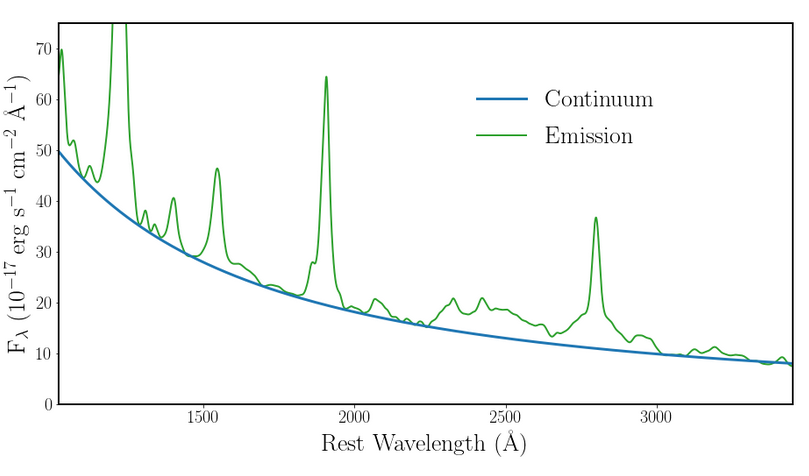
\includegraphics[width=\textwidth,height=4.16667in]{./Emission_Spectrum.png}
\caption{Quasar Spectrum}
\end{figure}

\hypertarget{galaxy-feedback}{%
\section{Galaxy Feedback}\label{galaxy-feedback}}

There's a well-known correlation between the mass of a galaxy's
spheroidal component and the mass of the supermassive black hole at its
center. For an elliptical galaxy, the spheroid is the whole galaxy, and
for a spiral galaxy the spheroid is the central bulge. A plot
illustrating this correlation is given below (Gültekin et al. (2009)).

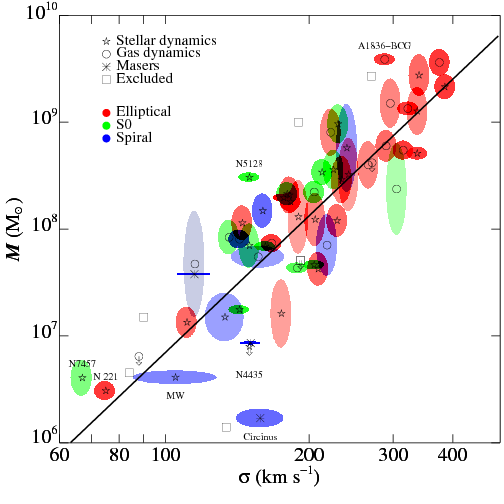
\includegraphics[width=\textwidth,height=4.16667in]{./msigma.png}

This is known as the M-\(\sigma\) relation. The x-axis is the host
galaxy's velocity dispersion, an analogue for its mass. The y-axis is
the mass of the supermassive black hole at the center of the host
galaxy. This correlation implies some coevolution mechanism between the
supermassive black hole and its host galaxy. The source of this
mechanism is an important area of active research.

\hypertarget{reverberation-mapping}{%
\section{Reverberation Mapping}\label{reverberation-mapping}}

One of the ways we can constrain the mass of the supermassive black hole
is through AGN reverberation mapping. Because gas in the broad line
region orbits the black hole with Keplerian velocities, we can use
properties of the broad line region to constrain the black hole mass. To
achieve this we need to calculate two things, a characteristic radius of
the broad line region, and the velocity dispersion of the gas at that
radius. If we can constrain these two values, our supermassive black
hole mass can be given by the following equation.

\[M_{BH}=f\frac{Rv^2}{G}\]

Where R is the radius of the broad line region and \(v\) is the
characteristic velocity. \(f\) is a parameter that takes in to account
things like the inclination of the accretion disc and the geometry of
the broad line region. In practice, we are usually not able to constrain
these values for an individual quasar, for reasons we'll discuss below,
and so average \(f\) values are determined. \(<f>\) can actually be
calculated from the M-\(\sigma\) relation above. Reverberation mapping
is not the only way to constrain the mass of a supermassive black hole,
so we can use the line of best fit for M-\(\sigma\) values determined
through other means to constrain our \(<f>\) for reverberation mapped
objects. The next few sections will discuss how we determine the radius
and velocity of the broad line region.

\hypertarget{constraining-the-radius}{%
\subsection{Constraining the Radius}\label{constraining-the-radius}}

The broad line region contains clouds of gas orbiting the supermassive
black hole with Keplerian velocities. This gas is illuminated by the
continuum from the accretion disk and manifests itself through emission
lines in quasar spectra.

Quasars have been observed to have significant variability in their
continua. Because the broad line region is illuminated by the continuum
source, variability in the continuum will cause variability in the
emission lines. However, the variability in the emission lines will lag
behind the variability in the continuum source, as it takes light time
to travel from the accretion disk to the broad line region. By probing
the time lag between the variability in the continuum and the
variability in the emission lines, we can derive an estimate for the
distance from the accretion disk to the broad line region.

The time delay of the variability (\(\tau\)) is equal to the average
distance (R) divided by the speed of light (c)

\[\tau=\frac{R}{c}\]

In practice we can determine \(\tau\) by gathering light curves for the
continuum and some emission line and estimating the lag using cross
correlation (more on that later).

While we consider the accretion disk to be small enough to ignore
variations in the location of the continuum, the same can not be said
for the broad line region. I.e we can not treat the broad line region as
a single point. In fact, we observe ionization stratification in the
broad line region. That is, emission lines with higher ionization
potentials will probe radii closer to the accretion disk. The broad line
region is more ionized closer to the accretion disk.

\begin{figure}
\centering
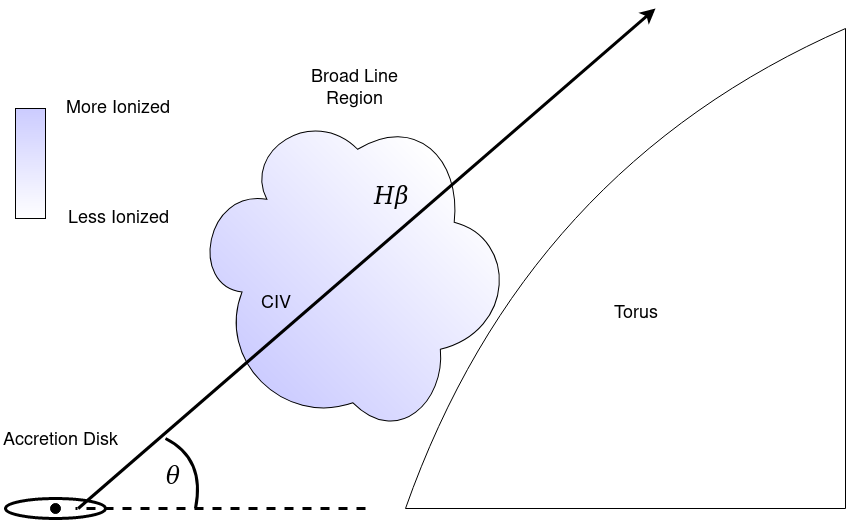
\includegraphics{./ReverberationMapping.png}
\caption{Reverberation Mapping Diagram}
\end{figure}

\hypertarget{transfer-function}{%
\subsubsection{Transfer Function}\label{transfer-function}}

When we pick out some emission line, like \(H\beta\) and use that, along
with the continuum, to measure \(\tau\), we are measuring the \(H\beta\)
emission weighted average light travel time. Continuum light travels
straight to the observer. The emission light will always take longer to
reach the observer than the continuum light, but, depending on where it
interacts with the broad line region, it can take any amount of time
longer to reach the observer.

\begin{figure}
\centering
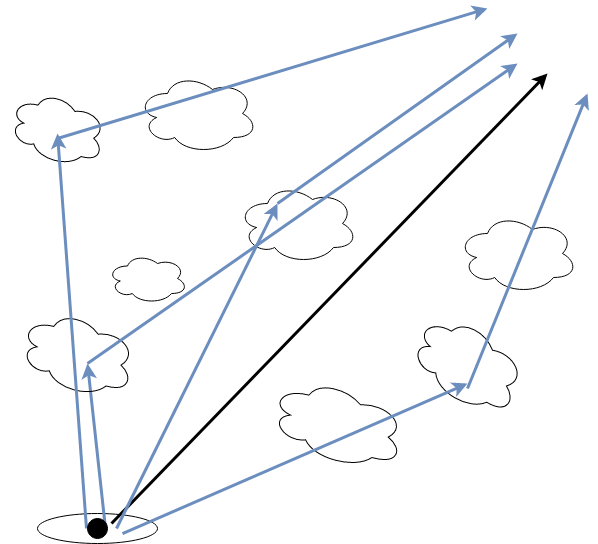
\includegraphics{./TransferFunction.png}
\caption{Emission Lag}
\end{figure}

When we observe a light curve for an emission line at a given time, we
are observing light that could have been emitted by the accretion disk
for all positive time delays. We can see how there needs to be some term
that gives us information about the geometry of the broad line region,
otherwise we would have no idea what radius we were probing. We call
this term the transfer function, \(\Psi(\tau)\), and it's defined such
that the emission light curve, L(t), is the convolution of the transfer
function and the continuum light curve, C(t)

\[L(t)=\int_{-\infty}^{\infty}\Psi(\tau)C(t-\tau)d\tau\]

We can think of this as the weighted average of the continuum light
curve given the geometry of the broad line region. More exactly, the
transfer function represents the broad line region's response to a
\(\delta\) function outburst, as observed from far away. Ideally, the
measurement of L(t) and C(t) would allow us to gain some information
about the geometry of the broad line region. However, there are many
reasons why this ends up being quite difficult. Most importantly, we are
often limited by the amount of data available (White and Peterson
(1994)).

In practice the transfer function is often ignored, and it is accepted
that black hole masses may be uncertain to a factor of \textasciitilde{}
2. Even considering the transfer function, you would still see a lag
value of \(\tau=\frac{R}{c}\) for both a thin spherical shell of radius
R and a thin ring of radius R at any inclination! (White and Peterson
(1994)).

\hypertarget{finding-the-lag}{%
\subsubsection{Finding the Lag}\label{finding-the-lag}}

In order to compute the lag time, we use the cross correlation function.
Cross correlation gives a measure of the similarity of two series as a
function of the displacement of one relative to the other.

\[F_{CCF}(\tau)=\int_{-\infty}^{\infty}L(t)C(t-\tau)dt\]

Let's examine the CCF for sin(x) and cos(x)

\includegraphics{./singif_screenshots/sinplots.gif}

The cross correlation function reaches its maximum at a delay of
\(3\pi/2\), when the two functions are identical. I.e
\(sin(x-3\pi/2)=cos(x)\).

We can plot our continuum and emission light curves with a delay and
find the lag time with the maximum cross correlation function value.
However, we have light curves sampled at discrete times, so we need a
discrete version of this cross correlation function.

\[F_{CCF}(\tau)=\frac{1}{N}\sum_{i=i}^N\frac{[L(t_i)-\bar L][C(t_i-\tau)-\bar C]}{\sigma_C \sigma_L}\]

White and Peterson (1994)

This method assumes evenly sampled time data, which is nearly impossible
to achieve, so we can interpolate our light curves onto evenly sampled
time intervals.

Once we've used the cross correlation function to pick out our ideal lag
time, we can determine the radius of the broad line region with

\[R=\tau c\]

\hypertarget{real-data}{%
\subsubsection{Real Data}\label{real-data}}

Let's look at some continuum and emission light curves. This data was
reported in Grier et al. (2012).

\begin{Shaded}
\begin{Highlighting}[]
\NormalTok{Continuum=}\KeywordTok{read.table}\NormalTok{(}\StringTok{"Mrk335_Continuum.txt"}\NormalTok{)}
\KeywordTok{colnames}\NormalTok{(Continuum)=}\KeywordTok{c}\NormalTok{(}\StringTok{"HJD"}\NormalTok{,}\StringTok{"Flux"}\NormalTok{)}
\KeywordTok{head}\NormalTok{(Continuum)}
\end{Highlighting}
\end{Shaded}

\begin{verbatim}
##        HJD  Flux
## 1 5431.450 6.010
## 2 5436.450 5.980
## 3 5438.460 6.040
## 4 5440.908 6.478
## 5 5441.869 6.196
## 6 5442.838 6.142
\end{verbatim}

\begin{Shaded}
\begin{Highlighting}[]
\NormalTok{Emission=}\KeywordTok{read.table}\NormalTok{(}\StringTok{"Mrk335_Emission.txt"}\NormalTok{)}
\KeywordTok{colnames}\NormalTok{(Emission)=}\KeywordTok{c}\NormalTok{(}\StringTok{"HJD"}\NormalTok{,}\StringTok{"FHb"}\NormalTok{)}
\KeywordTok{head}\NormalTok{(Emission)}
\end{Highlighting}
\end{Shaded}

\begin{verbatim}
##        HJD   FHb
## 1 5440.908 5.323
## 2 5441.869 5.496
## 3 5442.838 5.296
## 4 5444.840 5.287
## 5 5445.853 5.217
## 6 5447.924 5.264
\end{verbatim}

We'll want to normalize the flux values so they can be properly
compared.

\begin{Shaded}
\begin{Highlighting}[]
\NormalTok{normalize <-}\StringTok{ }\ControlFlowTok{function}\NormalTok{(x) \{}
    \KeywordTok{return}\NormalTok{ ((x }\OperatorTok{-}\StringTok{ }\KeywordTok{min}\NormalTok{(x)) }\OperatorTok{/}\StringTok{ }\NormalTok{(}\KeywordTok{max}\NormalTok{(x) }\OperatorTok{-}\StringTok{ }\KeywordTok{min}\NormalTok{(x)))}
\NormalTok{  \}}
\end{Highlighting}
\end{Shaded}

\begin{Shaded}
\begin{Highlighting}[]
\KeywordTok{library}\NormalTok{(ggplot2)}
\KeywordTok{ggplot}\NormalTok{()}\OperatorTok{+}
\StringTok{  }\KeywordTok{geom_line}\NormalTok{(}\KeywordTok{aes}\NormalTok{(HJD,}\KeywordTok{normalize}\NormalTok{(Flux)),}\DataTypeTok{data=}\NormalTok{Continuum)}\OperatorTok{+}
\StringTok{  }\KeywordTok{geom_line}\NormalTok{(}\KeywordTok{aes}\NormalTok{(HJD,}\KeywordTok{normalize}\NormalTok{(FHb)),}\DataTypeTok{data=}\NormalTok{Emission)}
\end{Highlighting}
\end{Shaded}

\includegraphics{ReverberationMapping_files/figure-latex/unnamed-chunk-6-1.pdf}

It's clear visually that these two light curves show similar
variability, with some time delay.

Now we can interpolate onto evenly sampled time bins

\begin{Shaded}
\begin{Highlighting}[]
\NormalTok{xout=}\KeywordTok{seq}\NormalTok{(}\KeywordTok{min}\NormalTok{(Emission}\OperatorTok{$}\NormalTok{HJD),}\KeywordTok{max}\NormalTok{(Emission}\OperatorTok{$}\NormalTok{HJD),}\DataTypeTok{length.out=}\KeywordTok{length}\NormalTok{(Emission}\OperatorTok{$}\NormalTok{HJD)) }\CommentTok{#pick evenly sampled x values}

\NormalTok{temp=}\KeywordTok{approx}\NormalTok{(Emission}\OperatorTok{$}\NormalTok{HJD,Emission}\OperatorTok{$}\NormalTok{FHb,xout) }\CommentTok{#interpolate emission light curve onto those values}
\NormalTok{temp=temp}\OperatorTok{$}\NormalTok{y}
\NormalTok{FHb_interp=}\KeywordTok{normalize}\NormalTok{(temp)}

\NormalTok{temp=}\KeywordTok{approx}\NormalTok{(Continuum}\OperatorTok{$}\NormalTok{HJD,Continuum}\OperatorTok{$}\NormalTok{Flux,xout) }\CommentTok{#interpolate continuum light curve onto those values}
\NormalTok{temp=temp}\OperatorTok{$}\NormalTok{y}
\NormalTok{Fc_interp=}\KeywordTok{normalize}\NormalTok{(temp)}

\KeywordTok{ggplot}\NormalTok{()}\OperatorTok{+}
\StringTok{  }\KeywordTok{geom_line}\NormalTok{(}\KeywordTok{aes}\NormalTok{(xout,Fc_interp))}\OperatorTok{+}
\StringTok{  }\KeywordTok{geom_line}\NormalTok{(}\KeywordTok{aes}\NormalTok{(xout,FHb_interp))}
\end{Highlighting}
\end{Shaded}

\includegraphics{ReverberationMapping_files/figure-latex/unnamed-chunk-7-1.pdf}

Now let's make a method for calculating the discrete cross correlation
function

\[F_{CCF}(\tau)=\frac{1}{N}\sum_{i=i}^N\frac{[L(t_i)-\bar L][C(t_i-\tau)-\bar C]}{\sigma_C \sigma_L}\]

\begin{Shaded}
\begin{Highlighting}[]
\NormalTok{CCF<-}\ControlFlowTok{function}\NormalTok{(C,L,x,lagmax)\{}
  
\NormalTok{  num_lags=lagmax }\CommentTok{#moving in intervals of 1}
\NormalTok{  N=}\KeywordTok{length}\NormalTok{(C)}

\NormalTok{  sigmaC=}\KeywordTok{sd}\NormalTok{(C)}
\NormalTok{  sigmaL=}\KeywordTok{sd}\NormalTok{(L)}
\NormalTok{  Cbar=}\KeywordTok{mean}\NormalTok{(C)}
\NormalTok{  Lbar=}\KeywordTok{mean}\NormalTok{(L)}
  
\NormalTok{  ccf_out=}\KeywordTok{c}\NormalTok{()}
\NormalTok{  lags=}\KeywordTok{c}\NormalTok{()}
  

  \ControlFlowTok{for}\NormalTok{(tau }\ControlFlowTok{in} \DecValTok{1}\OperatorTok{:}\NormalTok{lagmax)\{}
    
    
\NormalTok{    count=}\DecValTok{0} \CommentTok{#for normalization}
\NormalTok{    sum=}\DecValTok{0}

    \ControlFlowTok{for}\NormalTok{(i }\ControlFlowTok{in}\NormalTok{ (tau}\OperatorTok{+}\DecValTok{1}\NormalTok{)}\OperatorTok{:}\NormalTok{N)\{ }\CommentTok{#we have to cut off early values so C(t_i-tau) makes sense}
      
\NormalTok{      count=count}\OperatorTok{+}\DecValTok{1}

\NormalTok{      val=(L[i]}\OperatorTok{-}\NormalTok{Lbar)}\OperatorTok{*}\NormalTok{(C[i}\OperatorTok{-}\NormalTok{tau]}\OperatorTok{-}\NormalTok{Cbar)}\OperatorTok{/}\NormalTok{(sigmaC}\OperatorTok{*}\NormalTok{sigmaL) }\CommentTok{#discrete ccf for one i value}

\NormalTok{      sum=sum}\OperatorTok{+}\NormalTok{val}
\NormalTok{    \}}
    

\NormalTok{    ccf_out=}\KeywordTok{append}\NormalTok{(ccf_out,sum}\OperatorTok{/}\NormalTok{count)}
\NormalTok{    lags=}\KeywordTok{append}\NormalTok{(lags,x[tau]}\OperatorTok{-}\NormalTok{x[}\DecValTok{1}\NormalTok{])}
  
\NormalTok{  \}}

  
  \KeywordTok{return}\NormalTok{(}\KeywordTok{list}\NormalTok{(}\DataTypeTok{lags=}\NormalTok{lags,}\DataTypeTok{CCF=}\NormalTok{ccf_out))}
  
\NormalTok{\}}
\end{Highlighting}
\end{Shaded}

We can test this function on our sin and cos plot

\begin{Shaded}
\begin{Highlighting}[]
\NormalTok{x=}\KeywordTok{seq}\NormalTok{(}\OperatorTok{-}\DecValTok{2}\OperatorTok{*}\NormalTok{pi,}\DecValTok{2}\OperatorTok{*}\NormalTok{pi,}\DataTypeTok{length.out=}\DecValTok{50}\NormalTok{)}
\NormalTok{obj=}\KeywordTok{CCF}\NormalTok{(}\KeywordTok{sin}\NormalTok{(x),}\KeywordTok{cos}\NormalTok{(x),x,}\DecValTok{40}\NormalTok{)}

\KeywordTok{plot}\NormalTok{(obj}\OperatorTok{$}\NormalTok{lags,obj}\OperatorTok{$}\NormalTok{CCF,}\DataTypeTok{xlab=}\StringTok{'lag (radians)'}\NormalTok{,}\DataTypeTok{ylab=}\StringTok{'CCF'}\NormalTok{)}
\end{Highlighting}
\end{Shaded}

\includegraphics{ReverberationMapping_files/figure-latex/unnamed-chunk-9-1.pdf}

Again we see a peak at \(3\pi/2\).

Now let's apply it to our light curves

\begin{Shaded}
\begin{Highlighting}[]
\NormalTok{obj=}\KeywordTok{CCF}\NormalTok{(Fc_interp,FHb_interp,xout,}\DecValTok{30}\NormalTok{)}
\KeywordTok{plot}\NormalTok{(obj}\OperatorTok{$}\NormalTok{lags,obj}\OperatorTok{$}\NormalTok{CCF,}\DataTypeTok{xlab=}\StringTok{'lag (days)'}\NormalTok{,}\DataTypeTok{ylab=}\StringTok{'CCF'}\NormalTok{)}
\KeywordTok{lines}\NormalTok{(}\KeywordTok{c}\NormalTok{(}\DecValTok{15}\NormalTok{,}\DecValTok{15}\NormalTok{),}\KeywordTok{c}\NormalTok{(}\DecValTok{0}\NormalTok{,}\DecValTok{1}\NormalTok{))}
\end{Highlighting}
\end{Shaded}

\includegraphics{ReverberationMapping_files/figure-latex/unnamed-chunk-10-1.pdf}

Let's plot our continuum and emission light curves with variable lag
value, along with the CCF

\includegraphics{./laggif_screenshots/lagplots.gif}

Our final broad line region radius for this data is roughly 15 light
days. This is pretty consistent with the values reported in Grier et al.
(2012) for Mrk 335.

\hypertarget{constraining-the-velocity}{%
\subsection{Constraining the Velocity}\label{constraining-the-velocity}}

We determine the velocity dispersion of the broad line region by fitting
a single-epoch emission line for its velocity width. It's important to
remember that we must use the same emission line that we used to
constrain the radius, so we're probing the same region of the gas in the
broad line region. Often these values are measured with the H\(\beta\)
emission line.

\begin{Shaded}
\begin{Highlighting}[]
\KeywordTok{plot}\NormalTok{(WL,Flux)}
\end{Highlighting}
\end{Shaded}

\includegraphics{ReverberationMapping_files/figure-latex/unnamed-chunk-13-1.pdf}

For a simple application, we can fit the emission line with a Gaussian
profile (more accurately it should be a Voigt). Notice though that the
baseline is well above 0. We mentioned before that the continuum flux is
modelled as a power law, so we'll use that here. For a Gaussian

\[f(\lambda,\sigma,\mu)=A\frac{1}{\sigma\sqrt{2\pi}}e^{-\frac{1}{2}(\frac{\lambda-\mu}{\sigma})^2}\]

Where \(\lambda\) is the wavelength, A is the amplitude, \(\mu\) is the
mean and \(\sigma\) is the standard deviation.

And a power law is given by

\[f(\lambda)=C(\frac{\lambda}{\lambda_0})^{-\alpha}\]

Where C is the power law normalization and \(\alpha\) is the power law
slope. It's important to set \(\lambda_0\) to a value that's within the
band pass.

So our best fit is just the power law plus a gaussian. Let's define
these functions

\begin{Shaded}
\begin{Highlighting}[]
\CommentTok{#takes an array of wavelength values, as well as the mean and standard deviation, outputs an array of intensities}
\NormalTok{gauss<-}\ControlFlowTok{function}\NormalTok{(WL,mu,sigma,A)\{}
\NormalTok{  out=}\KeywordTok{c}\NormalTok{()}
  \ControlFlowTok{for}\NormalTok{(i }\ControlFlowTok{in} \DecValTok{1}\OperatorTok{:}\KeywordTok{length}\NormalTok{(WL))\{}
    
\NormalTok{    val=A}\OperatorTok{*}\NormalTok{(sigma}\OperatorTok{*}\KeywordTok{sqrt}\NormalTok{(}\DecValTok{2}\OperatorTok{*}\NormalTok{pi))}\OperatorTok{^}\NormalTok{(}\OperatorTok{-}\DecValTok{1}\NormalTok{)}\OperatorTok{*}\KeywordTok{exp}\NormalTok{(}\OperatorTok{-}\FloatTok{0.5}\OperatorTok{*}\NormalTok{((WL[i]}\OperatorTok{-}\NormalTok{mu)}\OperatorTok{/}\NormalTok{sigma)}\OperatorTok{^}\DecValTok{2}\NormalTok{)}
    
    
\NormalTok{    out=}\KeywordTok{append}\NormalTok{(out,val)}
\NormalTok{  \}}
  
  \KeywordTok{return}\NormalTok{(out)}
\NormalTok{\}}
\end{Highlighting}
\end{Shaded}

\begin{Shaded}
\begin{Highlighting}[]
\KeywordTok{plot}\NormalTok{(WL,}\KeywordTok{gauss}\NormalTok{(WL,}\DecValTok{4860}\NormalTok{,}\DecValTok{1}\NormalTok{,}\DecValTok{3}\NormalTok{))}
\end{Highlighting}
\end{Shaded}

\includegraphics{ReverberationMapping_files/figure-latex/unnamed-chunk-15-1.pdf}

\begin{Shaded}
\begin{Highlighting}[]
\CommentTok{#takes an array of wavelength values, as well as the powerlaw norm slope and lambda_0, outputs an array of intensities}
\NormalTok{powerlaw<-}\ControlFlowTok{function}\NormalTok{(WL,WL0,C,alpha)\{}
  
  \KeywordTok{return}\NormalTok{( C}\OperatorTok{*}\NormalTok{(WL}\OperatorTok{/}\NormalTok{WL0)}\OperatorTok{^}\NormalTok{(}\OperatorTok{-}\NormalTok{alpha)  )}
  
\NormalTok{\}}
\end{Highlighting}
\end{Shaded}

\begin{Shaded}
\begin{Highlighting}[]
\KeywordTok{plot}\NormalTok{(}\KeywordTok{powerlaw}\NormalTok{(WL,}\DecValTok{4840}\NormalTok{,}\DecValTok{9}\NormalTok{,}\FloatTok{1.4}\NormalTok{)}\OperatorTok{+}\KeywordTok{gauss}\NormalTok{(WL,}\DecValTok{4860}\NormalTok{,}\DecValTok{1}\NormalTok{,}\DecValTok{3}\NormalTok{))}
\end{Highlighting}
\end{Shaded}

\includegraphics{ReverberationMapping_files/figure-latex/unnamed-chunk-17-1.pdf}

Now we can try to match our model to the real data visually. We know
H\(\beta\) has a WL of 4861, so that's one less parameter to worry
about.

\begin{Shaded}
\begin{Highlighting}[]
\KeywordTok{library}\NormalTok{(ggplot2)}
\NormalTok{mu=}\DecValTok{4861}
\NormalTok{A_guess=}\DecValTok{8}
\NormalTok{sigma_guess=}\FloatTok{1.5}
\NormalTok{WL0=}\DecValTok{4840}
\NormalTok{C_guess=}\DecValTok{9}
\NormalTok{alpha_guess=}\FloatTok{0.8}

\NormalTok{model=}\KeywordTok{powerlaw}\NormalTok{(WL,WL0,C_guess,alpha_guess)}\OperatorTok{+}\KeywordTok{gauss}\NormalTok{(WL,mu,sigma_guess,A_guess)}


\KeywordTok{ggplot}\NormalTok{()}\OperatorTok{+}
\StringTok{  }\KeywordTok{geom_point}\NormalTok{(}\KeywordTok{aes}\NormalTok{(WL,Flux))}\OperatorTok{+}
\StringTok{  }\KeywordTok{geom_line}\NormalTok{(}\KeywordTok{aes}\NormalTok{(WL,model))}
\end{Highlighting}
\end{Shaded}

\includegraphics{ReverberationMapping_files/figure-latex/unnamed-chunk-18-1.pdf}

Now let's utilize a non-linear least squares fit to the data, to get
better estimates of fit parameters.

\begin{Shaded}
\begin{Highlighting}[]
\CommentTok{#coeff is a vector of fit parameters}
\NormalTok{WL0=}\DecValTok{4840}
\NormalTok{mu=}\DecValTok{4861}
\NormalTok{mod<-}\ControlFlowTok{function}\NormalTok{(WL,coeff)\{}
\NormalTok{  C_model=coeff[}\DecValTok{1}\NormalTok{]}
\NormalTok{  alpha_model=coeff[}\DecValTok{2}\NormalTok{]}
\NormalTok{  sigma_model=coeff[}\DecValTok{3}\NormalTok{]}
\NormalTok{  A_model=coeff[}\DecValTok{4}\NormalTok{]}
  
  \KeywordTok{powerlaw}\NormalTok{(WL,WL0,C_model,alpha_model)}\OperatorTok{+}\KeywordTok{gauss}\NormalTok{(WL,mu,sigma_model,A_model)}
  
\NormalTok{\}}


\NormalTok{obj=}\KeywordTok{nls}\NormalTok{(Flux }\OperatorTok{~}\StringTok{ }\KeywordTok{mod}\NormalTok{(WL,coef), }\DataTypeTok{start =} \KeywordTok{list}\NormalTok{(}\DataTypeTok{coef =} \KeywordTok{c}\NormalTok{(C_guess,alpha_guess,sigma_guess,A_guess)))}
\NormalTok{obj}
\end{Highlighting}
\end{Shaded}

\begin{verbatim}
## Nonlinear regression model
##   model: Flux ~ mod(WL, coef)
##    data: parent.frame()
## coef1 coef2 coef3 coef4 
## 9.001 1.841 1.010 5.044 
##  residual sum-of-squares: 2.853
## 
## Number of iterations to convergence: 5 
## Achieved convergence tolerance: 9.062e-06
\end{verbatim}

Now we can plot the model fit

\begin{Shaded}
\begin{Highlighting}[]
\NormalTok{coeff_nls=}\KeywordTok{c}\NormalTok{(}\FloatTok{9.001}\NormalTok{,}\FloatTok{1.841}\NormalTok{,}\FloatTok{1.010}\NormalTok{,}\FloatTok{5.044}\NormalTok{)}

\KeywordTok{ggplot}\NormalTok{()}\OperatorTok{+}
\StringTok{  }\KeywordTok{geom_point}\NormalTok{(}\KeywordTok{aes}\NormalTok{(WL,Flux))}\OperatorTok{+}
\StringTok{  }\KeywordTok{geom_line}\NormalTok{(}\KeywordTok{aes}\NormalTok{(WL,}\KeywordTok{mod}\NormalTok{(WL,coeff_nls)))}
\end{Highlighting}
\end{Shaded}

\includegraphics{ReverberationMapping_files/figure-latex/unnamed-chunk-20-1.pdf}

So our estimate of \(\sigma\) is 1.01. From this we can extract the
velocity width

\[FWHM (km/s)=\frac{c*2.355\sigma}{\lambda}\]

Where here \(\lambda\) is the wavelength of the transition at zero
velocity.

\begin{Shaded}
\begin{Highlighting}[]
\NormalTok{FWHM=(}\FloatTok{3e6}\OperatorTok{*}\FloatTok{2.355}\OperatorTok{*}\FloatTok{1.01}\NormalTok{)}\OperatorTok{/}\DecValTok{4861}
\NormalTok{FWHM}
\end{Highlighting}
\end{Shaded}

\begin{verbatim}
## [1] 1467.939
\end{verbatim}

So a representational velocity is 1468 km/s, this is also comparable to
reported values (Grier et al. (2012)).

\hypertarget{calculating-the-mass-of-the-black-hole}{%
\subsection{Calculating the Mass of the Black
Hole}\label{calculating-the-mass-of-the-black-hole}}

Returning to our equation

\[M_{BH}=\frac{<f>Rv^2}{G}\]

The AGN black hole mass database (below) uses \(<f>=4.3\). Therefore our
black hole mass, in solar masses, is given by

\begin{Shaded}
\begin{Highlighting}[]
\NormalTok{lightdays_to_km=}\FloatTok{2.59e10}
\NormalTok{m_to_km=}\DecValTok{1}\OperatorTok{/}\DecValTok{1000}
\NormalTok{kg_to_Msun=}\DecValTok{1}\OperatorTok{/}\FloatTok{1.989e30}
\NormalTok{Mbh=(}\FloatTok{4.3}\OperatorTok{*}\DecValTok{15}\OperatorTok{*}\NormalTok{lightdays_to_km}\OperatorTok{*}\DecValTok{1468}\OperatorTok{^}\DecValTok{2}\NormalTok{)}\OperatorTok{/}\NormalTok{(}\FloatTok{6.674e-11}\OperatorTok{*}\NormalTok{m_to_km}\OperatorTok{^}\DecValTok{3}\NormalTok{)}\OperatorTok{*}\NormalTok{kg_to_Msun}
\NormalTok{Mbh}
\end{Highlighting}
\end{Shaded}

\begin{verbatim}
## [1] 27120057
\end{verbatim}

\(M_{BH}=27x10^6\) is within the uncertainty presented in Grier et al.
(2012).

\hypertarget{black-hole-masses}{%
\section{Black Hole Masses}\label{black-hole-masses}}

The AGN black hole mass database has compiled all published
spectroscopic reverberation mapping studies of active galaxies, they
have currently published 62 black hole masses

\begin{Shaded}
\begin{Highlighting}[]
\NormalTok{mbh=}\KeywordTok{read.csv}\NormalTok{(}\StringTok{"MBH_edit.csv"}\NormalTok{,}\DataTypeTok{sep=}\StringTok{","}\NormalTok{,}\DataTypeTok{header=}\NormalTok{F)}
\KeywordTok{colnames}\NormalTok{(mbh)=}\KeywordTok{c}\NormalTok{(}\StringTok{"Name"}\NormalTok{,}\StringTok{"RA"}\NormalTok{,}\StringTok{"Dec"}\NormalTok{,}\StringTok{"redshift"}\NormalTok{,}\StringTok{"logMBH"}\NormalTok{,}\StringTok{"+elogMBH"}\NormalTok{,}\StringTok{"-elogMBH"}\NormalTok{)}
\KeywordTok{head}\NormalTok{(mbh)}
\end{Highlighting}
\end{Shaded}

\begin{verbatim}
##         Name         RA       Dec redshift   logMBH   +elogMBH   -elogMBH
## 1     Mrk335 00:06:19.5 +20:12:10  0.02579 7.230111 0.04168351 0.04407856
## 2    Mrk1501 00:10:31.0 +10:58:30  0.08934 8.066634 0.11930877 0.16504565
## 3 PG0026+129 00:29:13.6 +13:16:03  0.14200 8.486820 0.09559916 0.11910148
## 4 PG0052+251 00:54:52.1 +25:25:38  0.15445 8.461728 0.08276698 0.09424687
## 5   Fairall9 01:23:45.8 -58:48:21  0.04702 8.298947 0.07838917 0.11588266
## 6     Mrk590 02:14:33.5 -00:46:00  0.02639 7.569731 0.06181738 0.07425541
\end{verbatim}

\begin{Shaded}
\begin{Highlighting}[]
\KeywordTok{hist}\NormalTok{(mbh}\OperatorTok{$}\NormalTok{logMBH)}
\end{Highlighting}
\end{Shaded}

\includegraphics{ReverberationMapping_files/figure-latex/unnamed-chunk-24-1.pdf}

\hypertarget{template-shiny-application}{%
\section{Template shiny application}\label{template-shiny-application}}

Use this template to develop your own interactive applications

\begin{Shaded}
\begin{Highlighting}[]
\KeywordTok{library}\NormalTok{(shiny)}

\KeywordTok{shinyApp}\NormalTok{(}

\NormalTok{  ui <-}\StringTok{ }\KeywordTok{fluidPage}\NormalTok{(}
    
    \CommentTok{# App title }
    \KeywordTok{titlePanel}\NormalTok{(}\StringTok{"Template"}\NormalTok{),}
    
    \CommentTok{#Sidebar layout with input and output}
    \KeywordTok{sidebarLayout}\NormalTok{(}
      
      \CommentTok{#sidebar panel for inputs}
      \KeywordTok{sidebarPanel}\NormalTok{(}
        
        \CommentTok{#Input: Slider for tau}
        \KeywordTok{sliderInput}\NormalTok{(}\DataTypeTok{inputId=}\StringTok{"tau"}\NormalTok{,}
                    \DataTypeTok{label=}\StringTok{"lag:"}\NormalTok{,}
                    \DataTypeTok{min=}\DecValTok{0}\NormalTok{,}
                    \DataTypeTok{max=}\FloatTok{6.28}\NormalTok{,}
                    \DataTypeTok{value=}\DecValTok{0}\NormalTok{)),}
      
      \CommentTok{#Main panel for displaying outputs}
      \KeywordTok{mainPanel}\NormalTok{(}
        \KeywordTok{plotOutput}\NormalTok{(}\StringTok{"sinPlot"}\NormalTok{)}
  
\NormalTok{      )}
      
      
\NormalTok{    )}
    
\NormalTok{  ),}
  
  \CommentTok{## Server}
  
  \CommentTok{# Define a server function for the Shiny app}
  
\NormalTok{  server <-}\StringTok{ }\ControlFlowTok{function}\NormalTok{(input,output)\{}
    
\NormalTok{    output}\OperatorTok{$}\NormalTok{sinPlot <-}\StringTok{ }\KeywordTok{renderPlot}\NormalTok{(\{}
      \CommentTok{#plotting sin(x-tau)}
      
\NormalTok{      x=}\KeywordTok{seq}\NormalTok{(}\OperatorTok{-}\DecValTok{2}\OperatorTok{*}\NormalTok{pi,}\DecValTok{2}\OperatorTok{*}\NormalTok{pi,}\DataTypeTok{length.out=}\DecValTok{50}\NormalTok{)}
\NormalTok{      y1=}\KeywordTok{sin}\NormalTok{(x}\OperatorTok{-}\NormalTok{input}\OperatorTok{$}\NormalTok{tau)}

      
      \KeywordTok{ggplot}\NormalTok{()}\OperatorTok{+}
\StringTok{        }\KeywordTok{geom_line}\NormalTok{(}\KeywordTok{aes}\NormalTok{(x,y1),}\DataTypeTok{colour=}\StringTok{'red'}\NormalTok{)}

  
\NormalTok{    \})}
    

      
      
\NormalTok{    \}}
\NormalTok{)}
\end{Highlighting}
\end{Shaded}

\includegraphics{./templategif_screenshots/template.gif}

\hypertarget{references}{%
\section*{References}\label{references}}
\addcontentsline{toc}{section}{References}

\hypertarget{refs}{}
\leavevmode\hypertarget{ref-Grier_2012}{}%
Grier, C. J., B. M. Peterson, R. W. Pogge, K. D. Denney, M. C. Bentz,
Paul Martini, S. G. Sergeev, et al. 2012. ``REVERBERATION MAPPING
RESULTS FOR FIVE SEYFERT 1 GALAXIES.'' \emph{The Astrophysical Journal}
755 (1). IOP Publishing: 60.
\url{https://doi.org/10.1088/0004-637x/755/1/60}.

\leavevmode\hypertarget{ref-Gultekin_2009}{}%
Gültekin, Kayhan, Douglas O. Richstone, Karl Gebhardt, Tod R. Lauer,
Scott Tremaine, M. C. Aller, Ralf Bender, et al. 2009.
``THEM-\(\upsigma\) ANDM-LRELATIONS IN GALACTIC BULGES, AND
DETERMINATIONS OF THEIR INTRINSIC SCATTER.'' \emph{The Astrophysical
Journal} 698 (1). IOP Publishing: 198--221.
\url{https://doi.org/10.1088/0004-637x/698/1/198}.

\leavevmode\hypertarget{ref-White_1994}{}%
White, Russell J., and Bradley M. Peterson. 1994. ``Comments on
Cross-Correlation Methodology in Variability Studies of Active Galactic
Nuclei.'' \emph{Publications of the Astronomical Society of the Pacific}
106 (August). IOP Publishing: 879. \url{https://doi.org/10.1086/133456}.


\end{document}
